%%
%% This is file `example_DarkConsole.tex',
%% generated with the docstrip utility.
%%
%% The original source files were:
%%
%% examples_kmbeamer.dtx  (with options: `DarkConsole')
%% Copyright (c) 2011-2013 Kazuki Maeda <kmaeda@users.sourceforge.jp>
%%
%% Distributable under the MIT License:
%% http://www.opensource.org/licenses/mit-license.php
%%

\documentclass[aspectratio=169]{beamer}
\usepackage{amsmath}
\usepackage{mathspec}
\usepackage{xeCJK}

\usepackage{minted}
\usemintedstyle{monokai}

\usepackage{xcolor}
\definecolor{archblue}{RGB}{23, 147, 209}

%\setmainfont[Mapping=tex-text]{Terminus (TTF)}
\setmonofont[Mapping=tex-text]{Terminus (TTF)}
%\setsansfont[Mapping=tex-text]{Terminus (TTF)}

%\usetheme{DarkConsole}

\setbeamertemplate{theorems}[normal font]

\title{\Large{Datascience 3.0}}
\subtitle{Introduction to Machine learning in Python}
\author{Nemanja Mićović \\ \texttt{nemanja\_micovic@matf.bg.ac.rs} \\ \texttt{machinelearning.matf.bg.ac.rs}}
\institute{Faculty of Mathematics, University of Belgrade}

% define the norm operator
\newcommand{\norm}[1]{\left\lVert#1\right\rVert}

\usepackage[utf8]{inputenc}
%\usepackage[serbian]{babel}

\AtBeginSection[]
{
    \begin{frame}<beamer>
        \frametitle{Table of contents}
        \tableofcontents[currentsection]
    \end{frame}
}

\begin{document}

\begin{frame}
    \maketitle
\end{frame}

\begin{frame}{Table of contents}
    \tableofcontents
\end{frame}

% -------------------------------------------------------------------------------------------------
\section{Machine learning introduction}
% -------------------------------------------------------------------------------------------------
\begin{frame}{About Machine learning}
    \begin{itemize}
        \item Field of Artificial Intelligence
        \item Very active research field today
        \item Has acomplished amazing results
        \item Built on multiple mathematical disciplines
    \end{itemize}
\end{frame}
% -------------------------------------------------------------------------------------------------
\begin{frame}{About Machine learning}
    Famous definition by Tom M. Mitchell
    \begin{itemize}
        \item A computer program is said to learn from \textbf{experience E}  with respect to some class of \textbf{tasks T}
            and \textbf{performance measure P} if its performance at tasks in T, as measured by P, improves with \textbf{experience E}
    \end{itemize}
    What is the goal of Machine learning?
    \begin{itemize}
        \item To create models able to generalize
        \item To give a theoretical base of generalization
        \item To solve a whole class of problems difficult for deterministic algorithms
    \end{itemize}
\end{frame}
% -------------------------------------------------------------------------------------------------
\begin{frame}{Some result of Machine learning}
    \begin{itemize}
        \item 1992 - TD-Gammon, computer program develoepd by Gerald Tesauro able to play backgammon
        \item 2011 - IBM's Watson wins in quiz \textit{Jeopardy!}
        \item 2012 - Google X creates system able to recognize cats on video recordings
        \item 2015 - Classification error for images reduced to 3.6\% (5-10\% is the error made by humans)
        \item 2016 - Google creates AlphaGo, agent able to play Go who beats the world champion 4:1
        \item 2017 - AlphaGo plays against its 2016 version and wins 100/100 games
    \end{itemize}
\end{frame}
% -------------------------------------------------------------------------------------------------
\begin{frame}{Applications of Machine learning}
    \begin{columns}
    \begin{column}{0.5\textwidth}
        \begin{itemize}
            \item Autonomous driving
            \item Bioinformatics
            \item Social networks
            \item Algorithm porfolio
            \item Playing video games
            \item Image classification
            \item Recognizing handwritting
            \item Natural language processing
            \item Generating optimization algorithms \cite{learning-to-learn}
            \item Generating images
        \end{itemize}
    \end{column}
    \begin{column}{0.5\textwidth}  %%<--- here
        \begin{itemize}
            \item Computer vision
            \item Detecting credit card frauds
            \item Data mining
            \item Medical assistance and assesment
            \item Marketing
            \item Targeted marketing
            \item Controlling robots
            \item Economy
            \item Speach recognition
            \item Recommendation systems
        \end{itemize}
    \end{column}
    \end{columns}
\end{frame}
% -------------------------------------------------------------------------------------------------
\begin{frame}{But why is it so successful and popular today?}
    \begin{itemize}
        \item There is serious amount of mathematics behind \cite{Murphy, Bishop, tibshirani, shalev-schwartz, vapnik}
        \item Today we have big amounts of data
        \item We also have graphical cards with thousands of processors
        \begin{itemize}
            \item They allow us to get extremely high levels of parallelization
        \end{itemize}
        \item Industry and academia complement each other
        \begin{itemize}
            \item Our meeting here today is the evidence of that :)
        \end{itemize}
    \end{itemize}
\end{frame}
% -------------------------------------------------------------------------------------------------
\begin{frame}{Types of machine learning}
    \begin{itemize}
        \item Supervised learning
        \item Unsupervised learning
        \item Reinforcement learning
    \end{itemize}
\end{frame}
% -------------------------------------------------------------------------------------------------
\section{Supervised learning}
\begin{frame}{Supervised learning}
    \begin{itemize}
        \item Our main focus today
        \item We are given attributes $x_1, x_2, ... x_n$
        \item Using them, we need to predict target variable $y$
        \item We want to create a model that will approximate $f(x_1, x_2, ..., x_n) = y$
        \item So we need to create a function $f' \approx f$
    \end{itemize}
\end{frame}
% -------------------------------------------------------------------------------------------------
\begin{frame}{Regression}
    \begin{itemize}
        \item Target variable $y$ is continuous
        \item Trying to predict temperature ($y$) using pressure ($x$)
    \end{itemize}

    \begin{center}
        \begin{figure}
            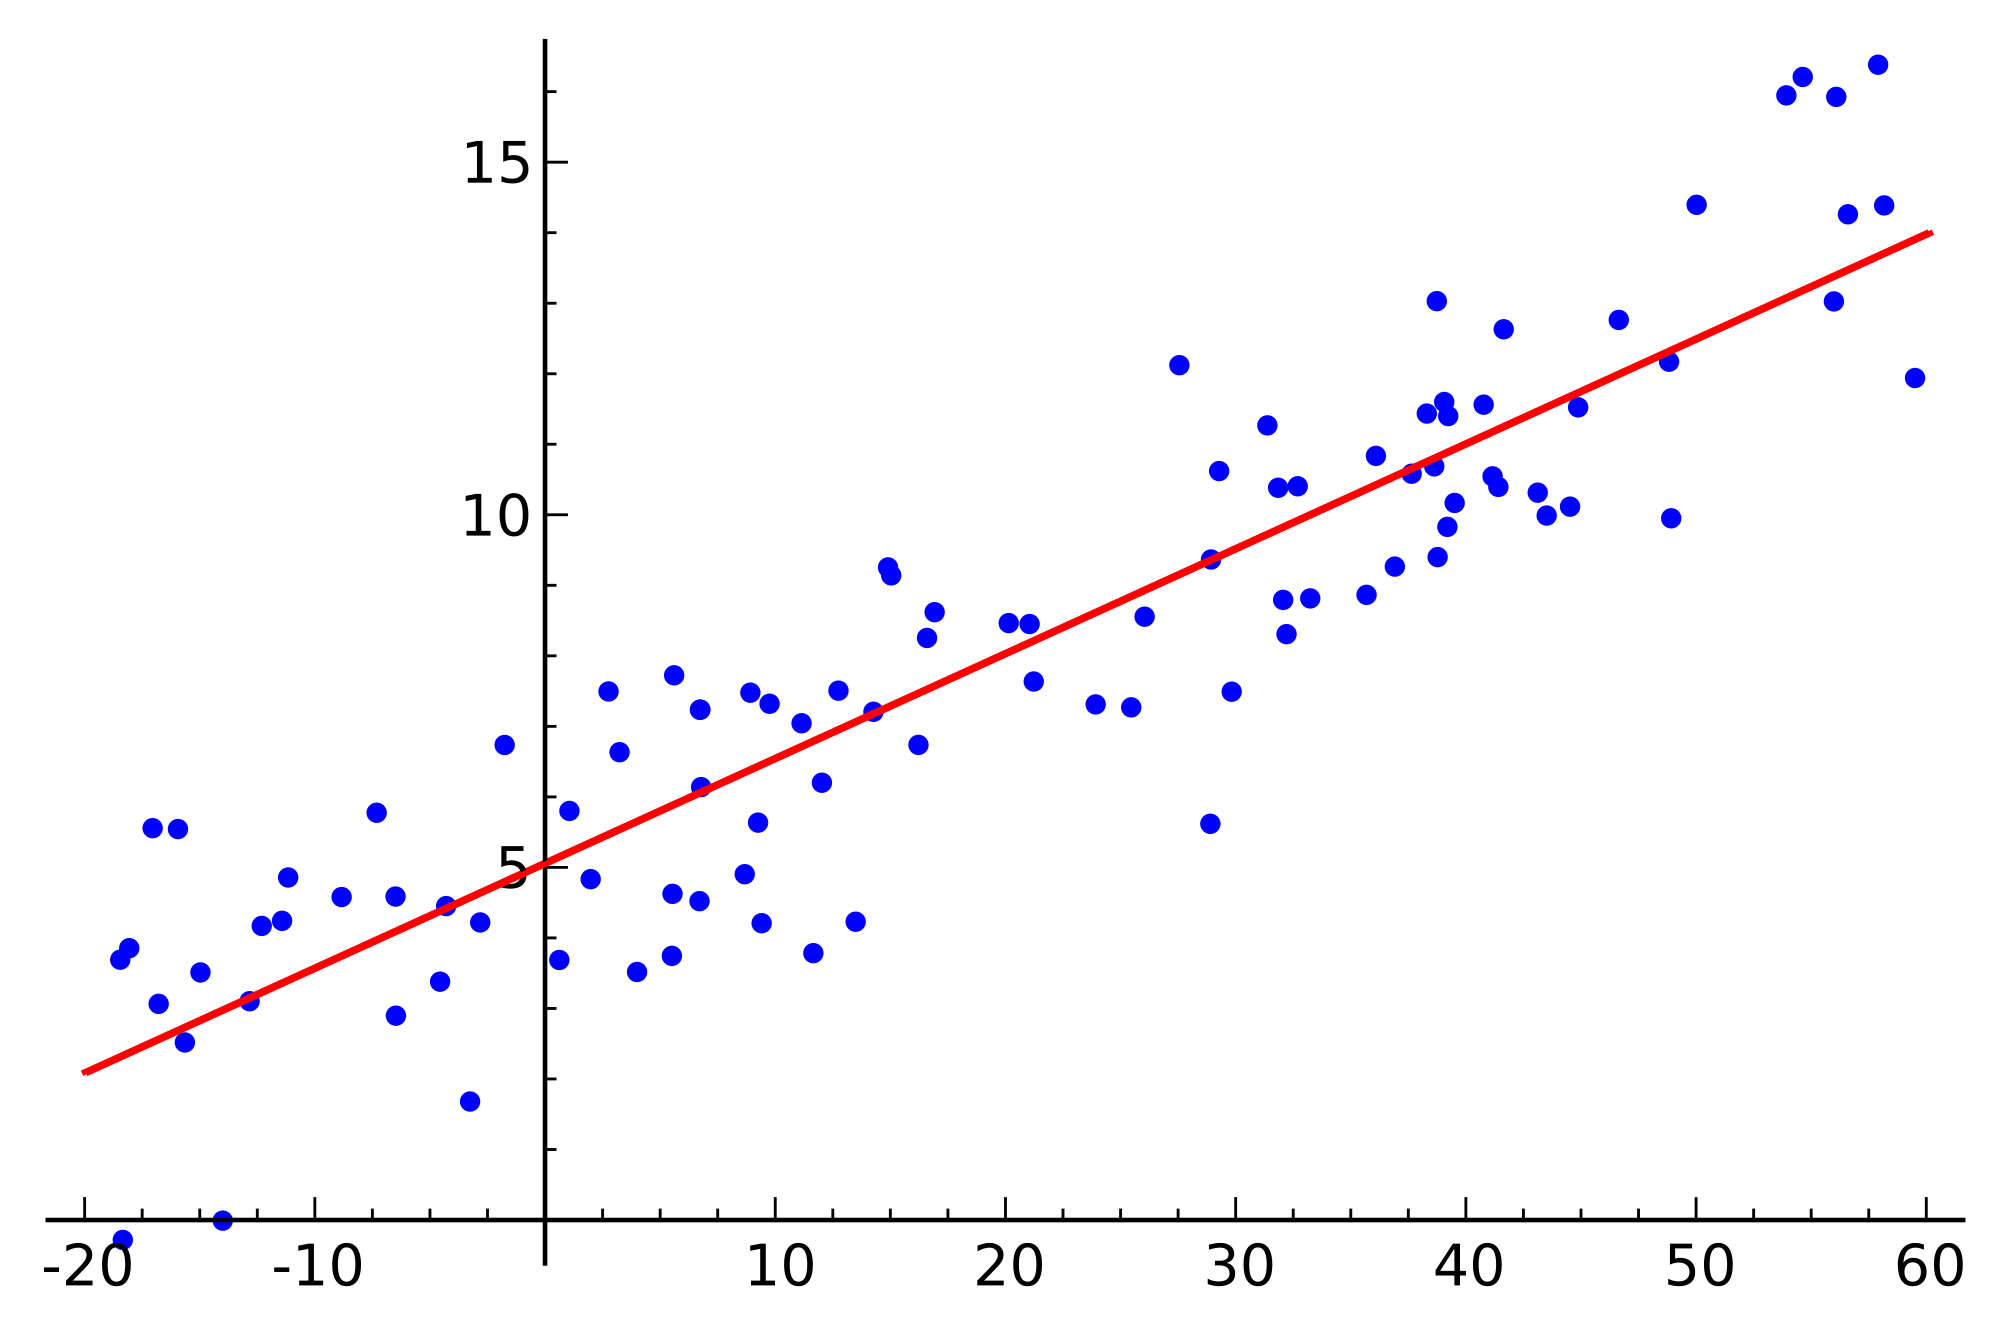
\includegraphics[scale=0.12]{./images/linear_regression.png}
            \caption{Linear regression (wikipedia)}
        \end{figure}
    \end{center}
\end{frame}
% -------------------------------------------------------------------------------------------------
\begin{frame}{Classification}
    \begin{itemize}
        \item Target variable $y$ is discreete
        \item Trying to predict gender ($y$) using weight ($x_1$) and height ($x_2$)
    \end{itemize}

    \begin{columns}
    \begin{column}{0.5\textwidth}
        \begin{center}
            \begin{figure}
                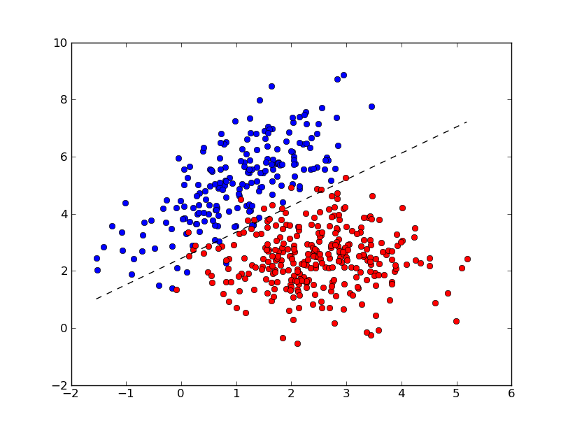
\includegraphics[scale=0.4]{./images/classification02.png}
                \caption{Classification example 1}
            \end{figure}
        \end{center}
    \end{column}
    \begin{column}{0.5\textwidth}  %%<--- here
        \begin{center}
            \begin{figure}
                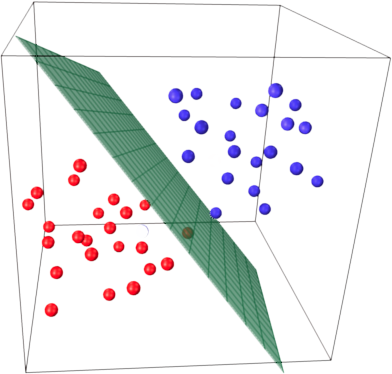
\includegraphics[scale=0.35]{./images/classification01.png}
                \caption{Classification example 2 (Sachin Joglekar's blog)}
            \end{figure}
        \end{center}
    \end{column}
    \end{columns}
\end{frame}
% -------------------------------------------------------------------------------------------------
\subsection{Linear regression}
% -------------------------------------------------------------------------------------------------
\begin{frame}{Linear regression}
    \begin{itemize}
        \item We construct the model in the following form:
        $$ f_w(x) = w_0 + w_1x_1 + w_2x_2 + ... + w_nx_n $$
        $$ f_w(x) = w_0 + \sum_{i=1}^{n} w_ix_i $$
    \item We calculate model accuracy using the following formula\footnote{Which is usually called \textit{Mean squared error}}:
        $$ Loss(w) = \frac{1}{N} \sum_{i=1}^{N} (y_i - f_w(x_i))^ 2 $$
    \end{itemize}
\end{frame}
% -------------------------------------------------------------------------------------------------
\begin{frame}{Linear regression - minimization problem}
    \begin{itemize}
        \item We have lots of different models
        \item Every tuple $(w_0, w_1, ..., w_n)$ defines a different model
        \item What is the \textit{best\footnote{Using term \textit{best} is tricky here, but let's stick with it for now.}} one?
        \item Model that makes the smallest mistake on the data we have is \textit{generally} great for us!
        \item But how do we find such model?
    \end{itemize}
\end{frame}
% -------------------------------------------------------------------------------------------------
\begin{frame}{Linear regression - minimization problem}
    \begin{itemize}
        \item Actually, that's not so difficult to do, we can derive the following equation with a bit of algebra
        \item Let's assume for simplicity that we have only one attribute $x$
        \item $x_i$ is the i-th dataset element
        \item $y_i$ is the target value for i-th dataset element
        $$ w = (X^\top X)^{-1}X^\top Y $$
        \[
        X =
          \begin{bmatrix}
            1 & x_1 \\
            1 & x_2 \\
            ... \\
            1 & x_N
          \end{bmatrix}
        Y =
          \begin{bmatrix}
            y_1 \\
            y_2 \\
            ... \\
            y_N
          \end{bmatrix}
        \]
    \end{itemize}
\end{frame}
% -------------------------------------------------------------------------------------------------
\begin{frame}{Linear regression - minimization problem}
    So what's the problem then?
    \begin{itemize}
        \item Matrix multiplication - lowest complexity so far $O(n^{2.373})$ \cite{fastmatrix}
        \item Matrix inverse - lowest complexity so far $O(n^{2.373})$
        \item Storing big\footnote{non sparse, we can store sparse matrices more efficiently} matrix $n \times m$ in memory:    $O(nm)$
    \end{itemize}
\end{frame}
% -------------------------------------------------------------------------------------------------
\begin{frame}{Linear regression - gradient descent}
    \begin{itemize}
        \item How does our error function generally look?
        \item Which point has the smaller error, $A$ or $B$?
    \end{itemize}
    \begin{center}
        \begin{figure}
            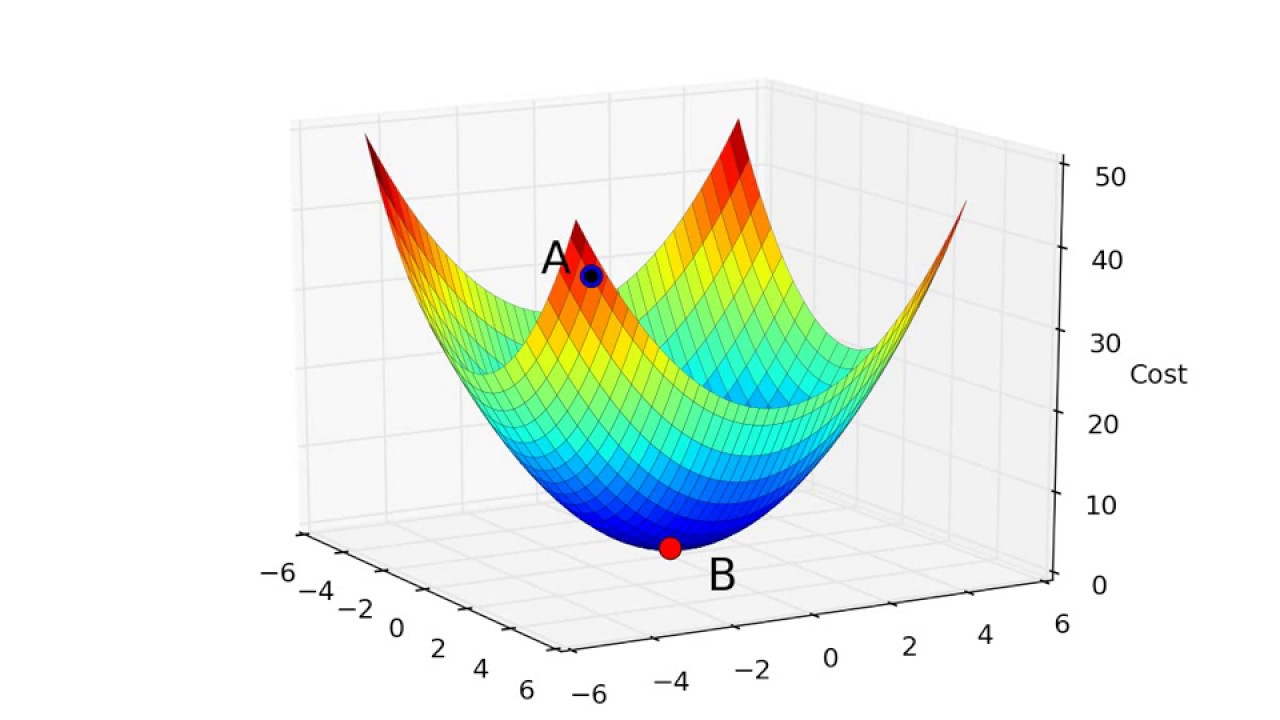
\includegraphics[scale=0.23]{./images/regressionGradient.jpg}
            \caption{An example of the error function}
        \end{figure}
    \end{center}
\end{frame}
% -------------------------------------------------------------------------------------------------
\begin{frame}{Linear regression - gradient descent}
    Can we somehow \textit{descend} into the function minimum?
    \begin{itemize}
        \item Yes!
    \end{itemize}
    But how?
    \begin{itemize}
        \item Calculate gradient of the error function with respect to $w$
        \item This vector \textit{points} into the direction of the fastest function growth
    \end{itemize}

    \begin{center}
        \begin{figure}
            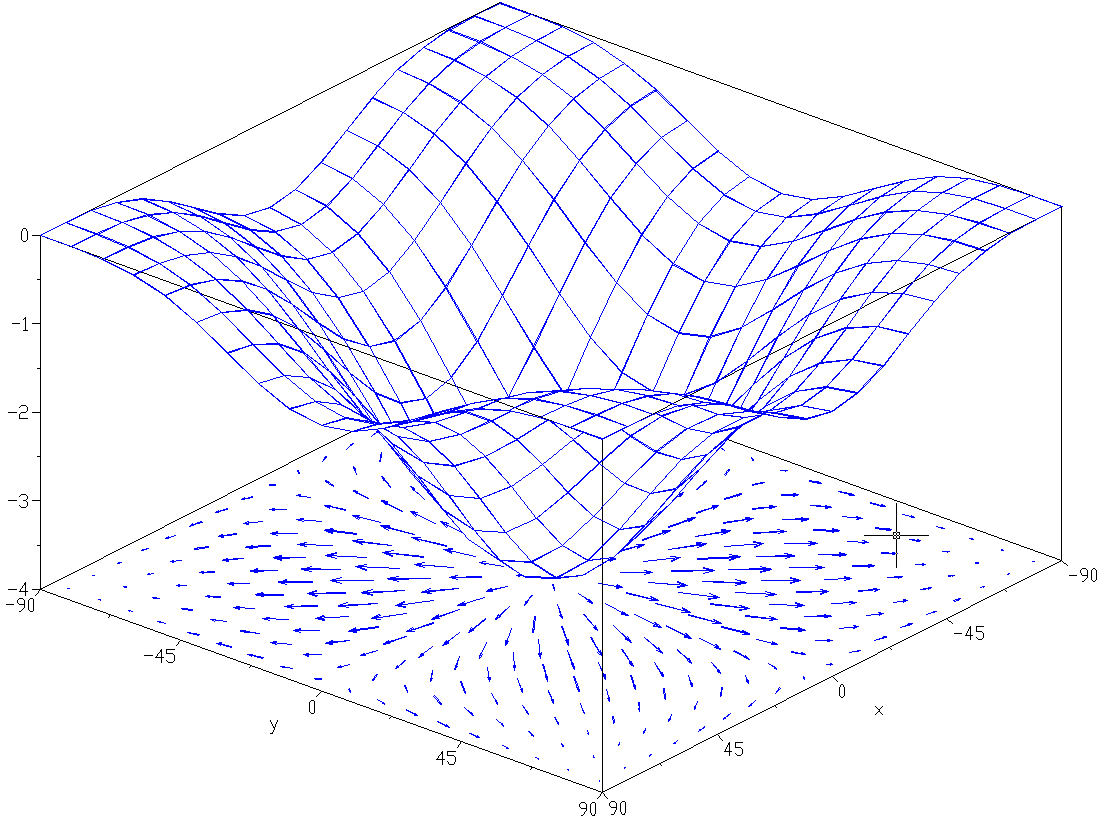
\includegraphics[scale=0.15]{./images/gradient.png}
            \caption{Blue arrows represent function gradients}
        \end{figure}
    \end{center}
\end{frame}
% -------------------------------------------------------------------------------------------------
\begin{frame}{Linear regression - gradient descent}
    Gradient descent algorithm:
    \begin{itemize}
        \item Repeat until convergence
        \begin{itemize}
            \item $ w_j := w_j - \mu \frac{\partial }{\partial w_j} Loss(w), \ j \in \{1, 2, ..., n\}  $
        \end{itemize}
    \end{itemize}

    \begin{center}
        \begin{figure}
            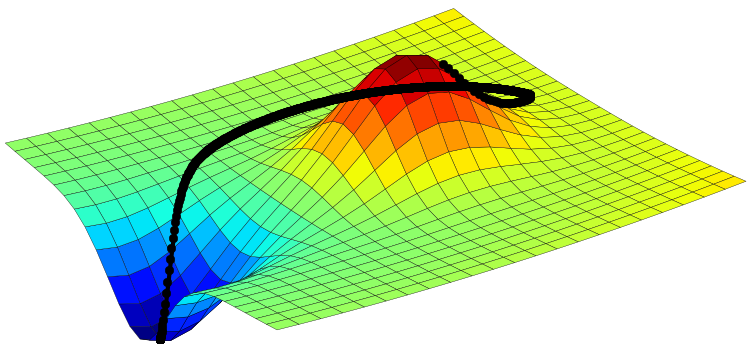
\includegraphics[scale=0.58]{./images/gradientDescent.png}
            \caption{An example of the steps made by the gradient descent algorithm (github.com/joshdk)}
        \end{figure}
    \end{center}
\end{frame}
% -------------------------------------------------------------------------------------------------
\begin{frame}{Linear regression - (R)MSE}
    \begin{itemize}
        \item Mean
            $$ \bar{y} = \frac{1}{N} \sum_{i=1}^{N} y_i $$
        \item Mean squared error (MSE)
        $$ \frac{1}{N} \sum_{i=1}^{N} (y_i - f_w(x_i))^ 2 $$
    \item Root mean squared error (RMSE)
        $$ \sqrt{\frac{1}{N} \sum_{i=1}^{N} (y_i - f_w(x_i))^ 2} $$
    \end{itemize}
\end{frame}
% -------------------------------------------------------------------------------------------------
\begin{frame}{Linear regression - $R^2$}
    \begin{itemize}
        \item Coefficient of determination, mostly called $R^2$
        \item It is the \textbf{proportion of the variation} in the \textbf{dependent}  variable that is predictable from the \textbf{independent} variable(s)
        \item We can say that it determines how much of variability has our model \textbf{managed to explain}
        \item What is the minimum of $R^2$?
        \item What is the maximum of $R^2$?
    \end{itemize}

    $$ R^2 = 1 - \frac{\sum_{i=1}^N(f_w(x_i) - y_i)^2}{\sum_{i=1}^N(\bar{y} - y_i)^2} $$
\end{frame}
% -------------------------------------------------------------------------------------------------
\begin{frame}{Linear regression - coding time}
    \begin{itemize}
        \item Let's code linear regression in \texttt{scikit-learn}
    \end{itemize}
\end{frame}
% -------------------------------------------------------------------------------------------------
\begin{frame}{Linear regression - overfitting}
    \begin{itemize}
        \item Analyze the following images\footnote{Images taken from book \textit{P. Janičić, M. Nikolić, Artificial Intelligence}}
    \end{itemize}
    \begin{columns}
    \begin{column}{0.5\textwidth}
        \begin{center}
            \begin{figure}
                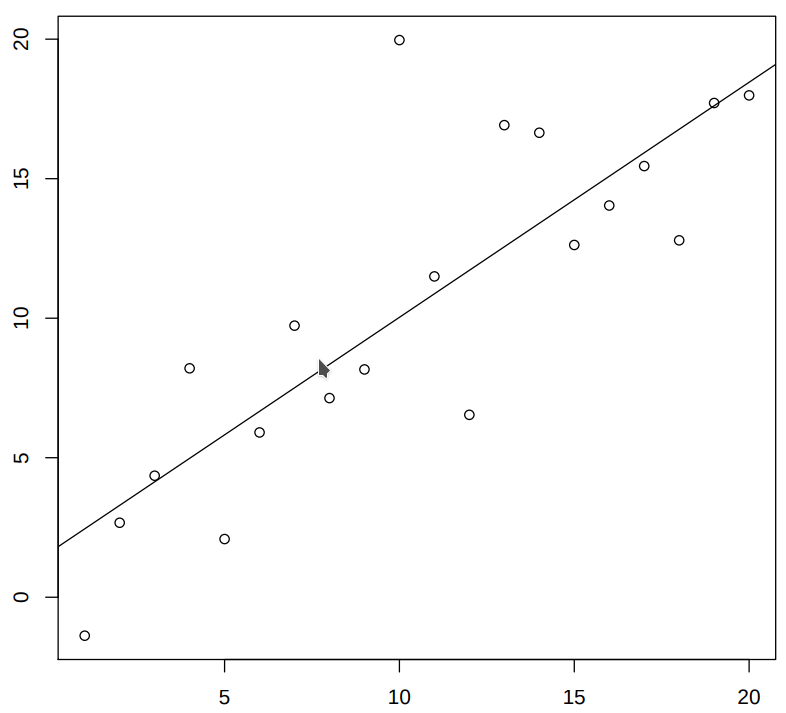
\includegraphics[scale=0.28]{./images/linreg.png}
                \caption{Linear regression 1}
            \end{figure}
        \end{center}
    \end{column}
    \begin{column}{0.5\textwidth}  %%<--- here
        \begin{center}
            \begin{figure}
                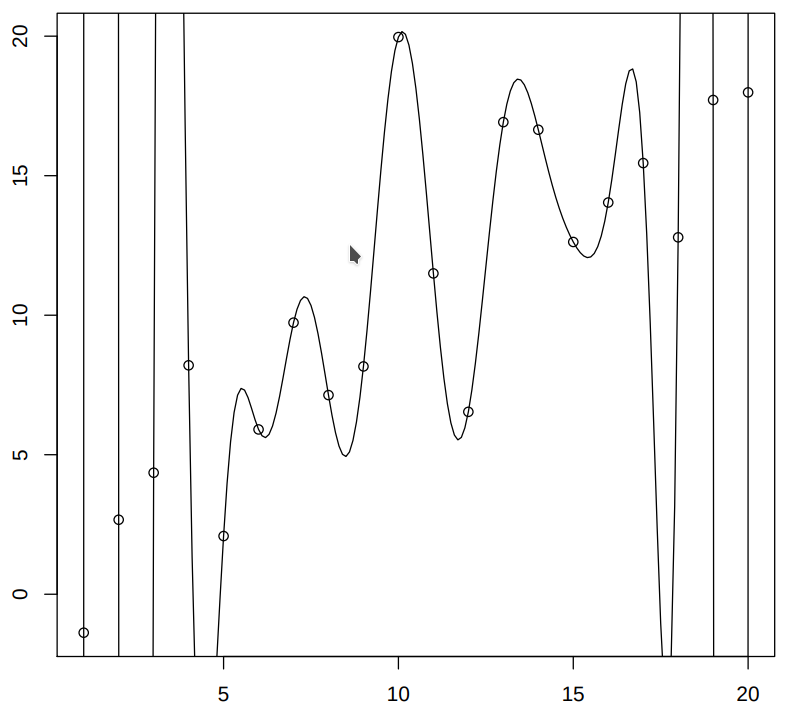
\includegraphics[scale=0.281]{./images/polyreg.png}
                \caption{Linear regression 2}
            \end{figure}
        \end{center}
    \end{column}
    \end{columns}
\end{frame}
% -------------------------------------------------------------------------------------------------
\begin{frame}{Linear regression - underfitting and overfitting}
    \begin{itemize}
        \item Given 3 models, which  one do you prefer in respect to black points (dataset samples)?
    \end{itemize}
    \begin{center}
        \begin{figure}
            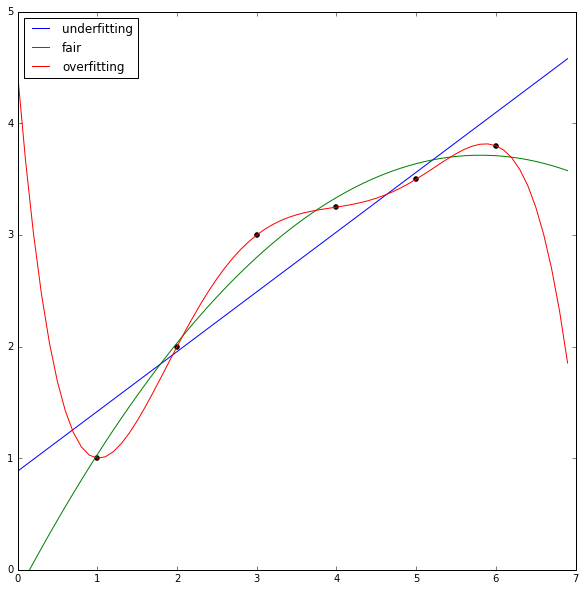
\includegraphics[scale=0.27]{./images/overunderfit.png}
            \caption{Examples of underfitting and overfitting}
        \end{figure}
    \end{center}
\end{frame}
% -------------------------------------------------------------------------------------------------
\begin{frame}{Linear regression - underfitting and overfitting}
    \textbf{Underfitting}
    \begin{itemize}
        \item A situation in which our model is not flexible enough in order
            to capture the essence of a phenomena
    \end{itemize}
    \textbf{Overfitting}
    \begin{itemize}
        \item A situation in which our model is too flexible and it fits too well
            towards the training data we feed it
    \end{itemize}
\end{frame}
% -------------------------------------------------------------------------------------------------
\begin{frame}{Linear regression - underfitting and overfitting}
    \begin{itemize}[<+->]
        \item If $MSE_{train} = 0$ , are we \textit{always} happy?
            \begin{itemize}
                \item Not really, we probably have overfitted quite a bit
            \end{itemize}
        \item If $MSE_{test} = 0$ , are we \textit{mostly} happy?
            \begin{itemize}
                \item Indeed we are, if we have a decent representable test set
            \end{itemize}
        \item If we have underfitting, which one will be bigger, $MSE_{train}$ or $MSE_{test}$?
            \begin{itemize}
                \item They will both be rather large
            \end{itemize}
        \item If we have overfitting, which one will be bigger, $MSE_{train}$ or $MSE_{test}$?
            \begin{itemize}
                \item $MSE_{test}$ > $MSE_{train}$
            \end{itemize}
    \end{itemize}
\end{frame}
% -------------------------------------------------------------------------------------------------
\begin{frame}{Linear regression - underfitting and overfitting}
    \begin{center}
        \begin{figure}
            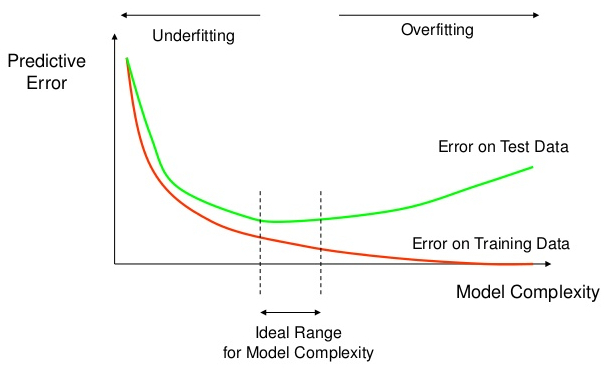
\includegraphics[scale=0.46]{./images/underoverfitGraph.jpg}
            \caption{Graph showing the difference between underfitting and overfitting}
        \end{figure}
    \end{center}
\end{frame}
% -------------------------------------------------------------------------------------------------
\begin{frame}{Linear regression - How to battle underfitting?}
    \begin{itemize}
        \item Take a more flexible model
        \item Instead of $f_w(x) = w_0 + w_1x_1 + x_2x_2$ take $g_w(x) = w_0 + w_1w_2x_1 + w_1^2x1 + w_2^2x2$
        \item Usually easier to solve then overfitting
        \item There is a wide variety of flexible models, and we can always complicate things\footnote{As in life and mathematics...}
    \end{itemize}
\end{frame}
% -------------------------------------------------------------------------------------------------
\begin{frame}{Linear regression - How to battle overfitting?}
    \textbf{Regularization}
    \begin{itemize}
        \item It allows us to control model complexity
        \item Term $\lambda$ controls the \textit{intensity} of regularization
        \item There are multiple options to pick from for function $\Omega$
        \item Interesting tutorial: https://www.analyticsvidhya.com/blog/2016/01/complete-tutorial-ridge-lasso-regression-python/
        \item We modify the minimization problem into:
    \end{itemize}
    $$ \min_w \frac{1}{N} \sum_{i=1}^{N} (y_i - f_w(x_i))^ 2 + \lambda \Omega(w) $$
\end{frame}
% -------------------------------------------------------------------------------------------------
\begin{frame}{Linear regression - Ridge regularization}
    \begin{itemize}
        \item Very commong regularization function
        \item It forces optimization algorithms not to increase model coefficients too much
        \item If coefficients get increased, then the sum of their squares rise a lot
        $$ \Omega(w) = \norm{w}_2^2 = \sum_{i=1}^{n}w_i^2 $$
    \item Using ridge, we obtain the following minimization problem
    $$ \min_w \frac{1}{N} \sum_{i=1}^{N} (y_i - f_w(x_i))^ 2 + \lambda \sum_{i=1}^{n}w_i^2 $$
    \end{itemize} 
\end{frame}
% -------------------------------------------------------------------------------------------------
\begin{frame}{Linear regression - coding time}
    \begin{itemize}
        \item Let's code ridge regression in \texttt{scikit-learn}
    \end{itemize}
\end{frame}
% -------------------------------------------------------------------------------------------------


% -------------------------------------------------------------------------------------------------
\subsection{K-Nearest neighbours}
% -------------------------------------------------------------------------------------------------
\begin{frame}{}
    \begin{center}
        \Large{\texttt{K-Nearest neighbours (kNN)}}
    \end{center}
\end{frame}
% -------------------------------------------------------------------------------------------------
\begin{frame}{kNN}
    \begin{itemize}
        \item Simple yet sometimes powerful classification algorithm
        \item \texttt{K} inside name comes from parameter $k$
        \item $k$ determines the number of neighbours we check when classifying an instance
    \end{itemize}
\end{frame}
% -------------------------------------------------------------------------------------------------
\begin{frame}{kNN}
    \begin{columns}
    \begin{column}{0.5\textwidth}
        \begin{itemize}[<+->]
            \item How much is $k$?
                \begin{itemize}
                    \item 5
                \end{itemize}
            \item What is the class of A?
                \begin{itemize}
                    \item Red
                \end{itemize}
            \item What is the class of B?
                \begin{itemize}
                    \item Red
                \end{itemize}
        \end{itemize}
    \end{column}
    \begin{column}{0.5\textwidth}  %%<--- here
        \begin{center}
            \begin{figure}
                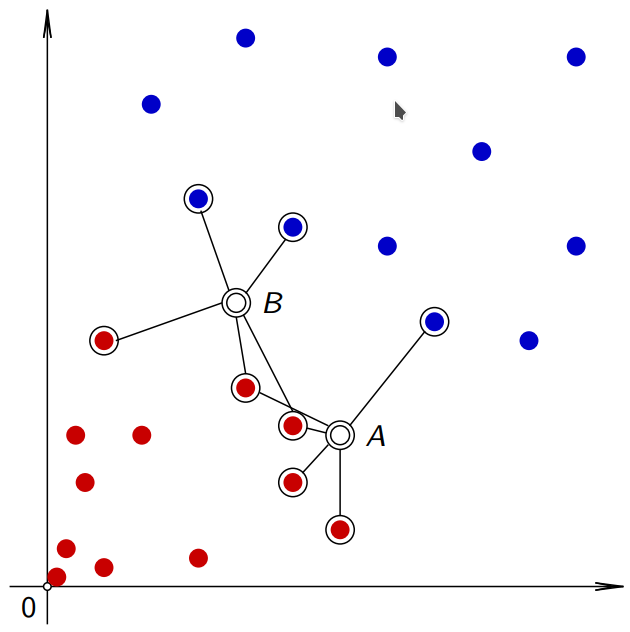
\includegraphics[scale=0.33]{./images/knn.png}
            \caption{kNN example (image taken from \cite{vi}}
            \end{figure}
        \end{center}
    \end{column}
    \end{columns}
\end{frame}
% -------------------------------------------------------------------------------------------------
\begin{frame}{kNN}
    \begin{center}
        \begin{figure}
            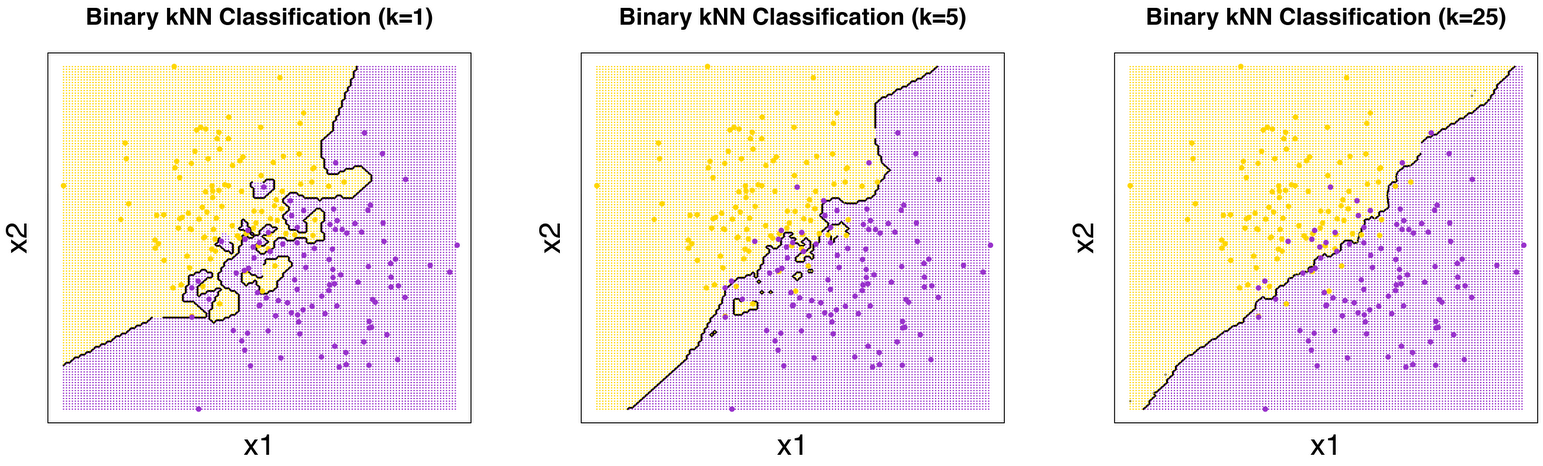
\includegraphics[scale=0.27]{./images/knn02.png}
        \caption{kNN example (image taken from Burton DeWilde's blog}
        \end{figure}
    \end{center}
\end{frame}
% -------------------------------------------------------------------------------------------------
\begin{frame}{kNN}
    \begin{itemize}[<+->]
        \item In linear regression, we represented our model with coefficients $w$
        \item What is the  model in the kNN classifier?
            \begin{itemize}
                \item There is no such thing, we only need to know $k$
            \end{itemize}
        \item How do we train the model?
            \begin{itemize}
                \item We don't, but every time we must calculate neighbours for a new instance
            \end{itemize}
    \end{itemize}
\end{frame}
% -------------------------------------------------------------------------------------------------
\begin{frame}{kNN - distances}
    \begin{itemize}
        \item There are multiple functions we can use to calculate distances
        \item Assume we are given points $x = (x_1, ..., x_n)$ and $y = (y_1, ..., y_n)$
        \item Minkowski
            $$ \bigg( {\sum_{i=1}^{n} (|x_i - y_i|)^q} \bigg)^\frac{1}{q} $$
        \item Manhattan (q = 1)
            $$ \sum_{i=1}^{n} \left| x_i - y_i \right| $$
        \item Euclidean distance (q = 2)
            $$ \sqrt{\sum_{i=1}^{n} (x_i - y_i)^2} $$
    \end{itemize}
\end{frame}
% -------------------------------------------------------------------------------------------------
\begin{frame}{kNN - Curse of dimensionality}
    \begin{itemize}
        \item Our intuition is bad for high dimensionals spaces
        \item When dimensionality increases, the volume of space increases really fast
        \item This can make our dataset very sparse
        \item Essentially, we number of dataset instances required increases exponentially with the dimensionality
        \item This is very bad for kNN
    \end{itemize}
\end{frame}
% -------------------------------------------------------------------------------------------------
\begin{frame}{Classification - important metrics}
    \begin{itemize}
        \item TP (true positive): those that are positive and our model was correct
        \item TN (true negative): those that are negative and our model was correct
        \item FP (false positive): those that are negative and our model was wrong
        \item FN (false negative): those that are negative and our model was wrong
        \item \textit{Accuracy}
            $$ Acc = \frac{TP + TN}{TP + TN + FP + FN} $$
        \item \textit{Precision}
            $$ Precision = \frac{TP}{TP + FP} $$
        \item \textit{Recall} score
            $$ Recall = \frac{TP}{TP + FN} $$
        \item $F_1$ score
            $$ F_1 = \frac{2TP}{2TP + FP + FN} $$
    \end{itemize}
\end{frame}

% -------------------------------------------------------------------------------------------------
\subsection{Logistic regression}
% -------------------------------------------------------------------------------------------------
\begin{frame}{}
    \begin{center}
        \Large{\texttt{Logistic regression}}
    \end{center}
\end{frame}
% -------------------------------------------------------------------------------------------------
\begin{frame}{Logistic regression}
    \begin{itemize}
        \item Classification algorithm
        \item By design, similar to linear regression
        \item We want to approximate $p(y|x)$
        $$ f_w(x) = w_0 + \sum_{i=1}^{n} w_i x_i $$
        \item $f_w(x)$ is not in interval $[0, 1]$
    \end{itemize}
\end{frame}
% -------------------------------------------------------------------------------------------------
\begin{frame}{Logistic regression - sigmoid function}
    $$ \sigma(x) = \frac{1}{1 + e^{-x}} $$
    \begin{center}
        \begin{figure}
            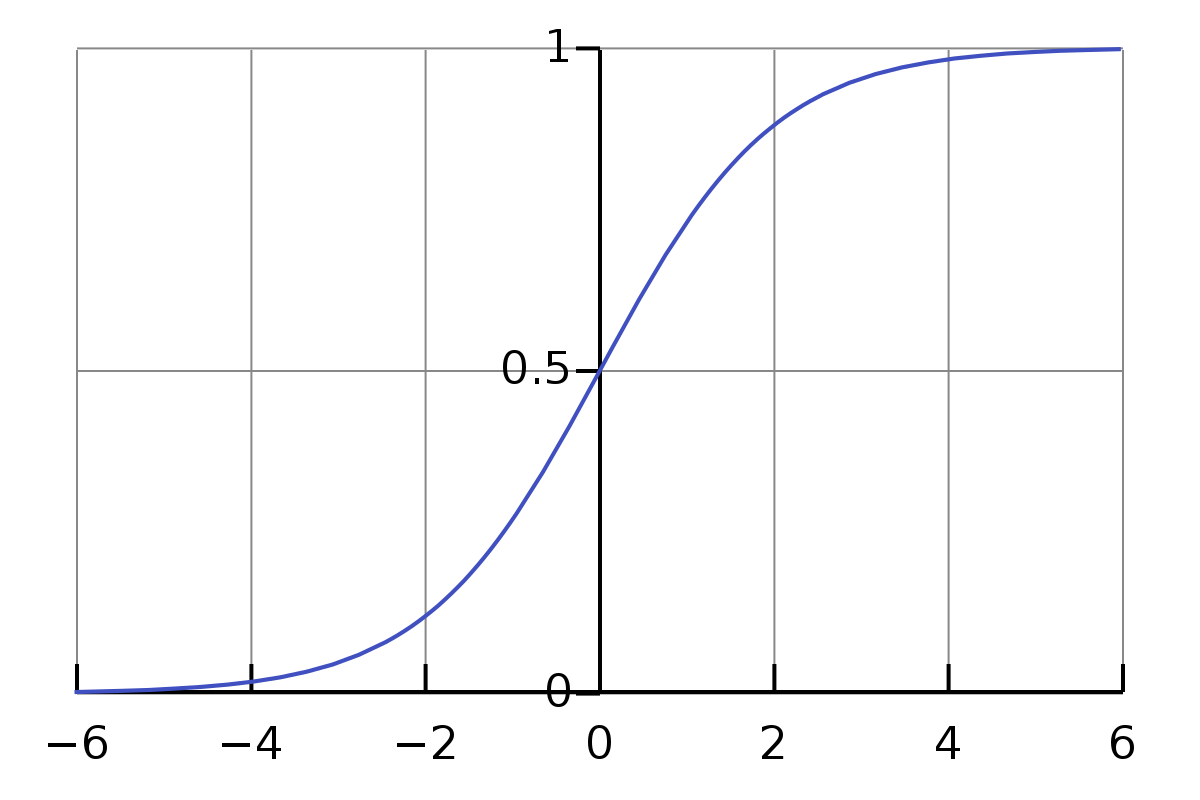
\includegraphics[scale=0.2]{./images/sigmoid.png}
            \caption{Graph of the sigmoid function}
        \end{figure}
    \end{center}
\end{frame}
% -------------------------------------------------------------------------------------------------
\begin{frame}{Logistic regression - loss function}
    \begin{itemize}
        \item We define the loss function as following (check \cite{Bishop, Murphy} for details)
    \end{itemize}

    $$
    Loss(w) = - \sum_{i=1}{N}\log p_w(y_i|x_i) = - \sum_{i=1}^{N}[y_i \log f_w(x_i) + (1 - y_i)\log (1-f_w(x_i))]
    $$
\end{frame}
% -------------------------------------------------------------------------------------------------
\begin{frame}{Logistic regression - minimization problem}
    \begin{itemize}
        \item We end up with the following minimization problem
    \end{itemize}
    $$
    \min_w - \sum_{i=1}^{N}[y_i \log f_w(x_i) + (1 - y_i)\log (1-f_w(x_i))]
    $$
    \begin{itemize}
        \item Which is a convex function with a global minimum
    \end{itemize}
\end{frame}
% -------------------------------------------------------------------------------------------------
\begin{frame}{Logistic regression - examples}
    \begin{columns}
    \begin{column}{0.5\textwidth}
        \begin{center}
            \begin{figure}
                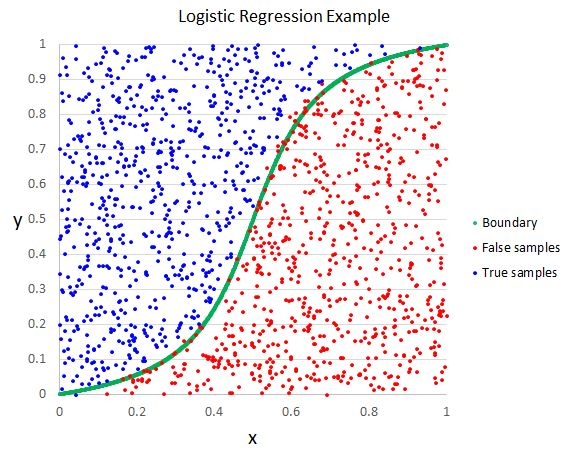
\includegraphics[scale=0.4]{./images/logisticRegression01.jpg}
            \caption{Example taken from www.helloacm.com}
            \end{figure}
        \end{center}
    \end{column}
    \begin{column}{0.5\textwidth}  %%<--- here
        \begin{center}
            \begin{figure}
                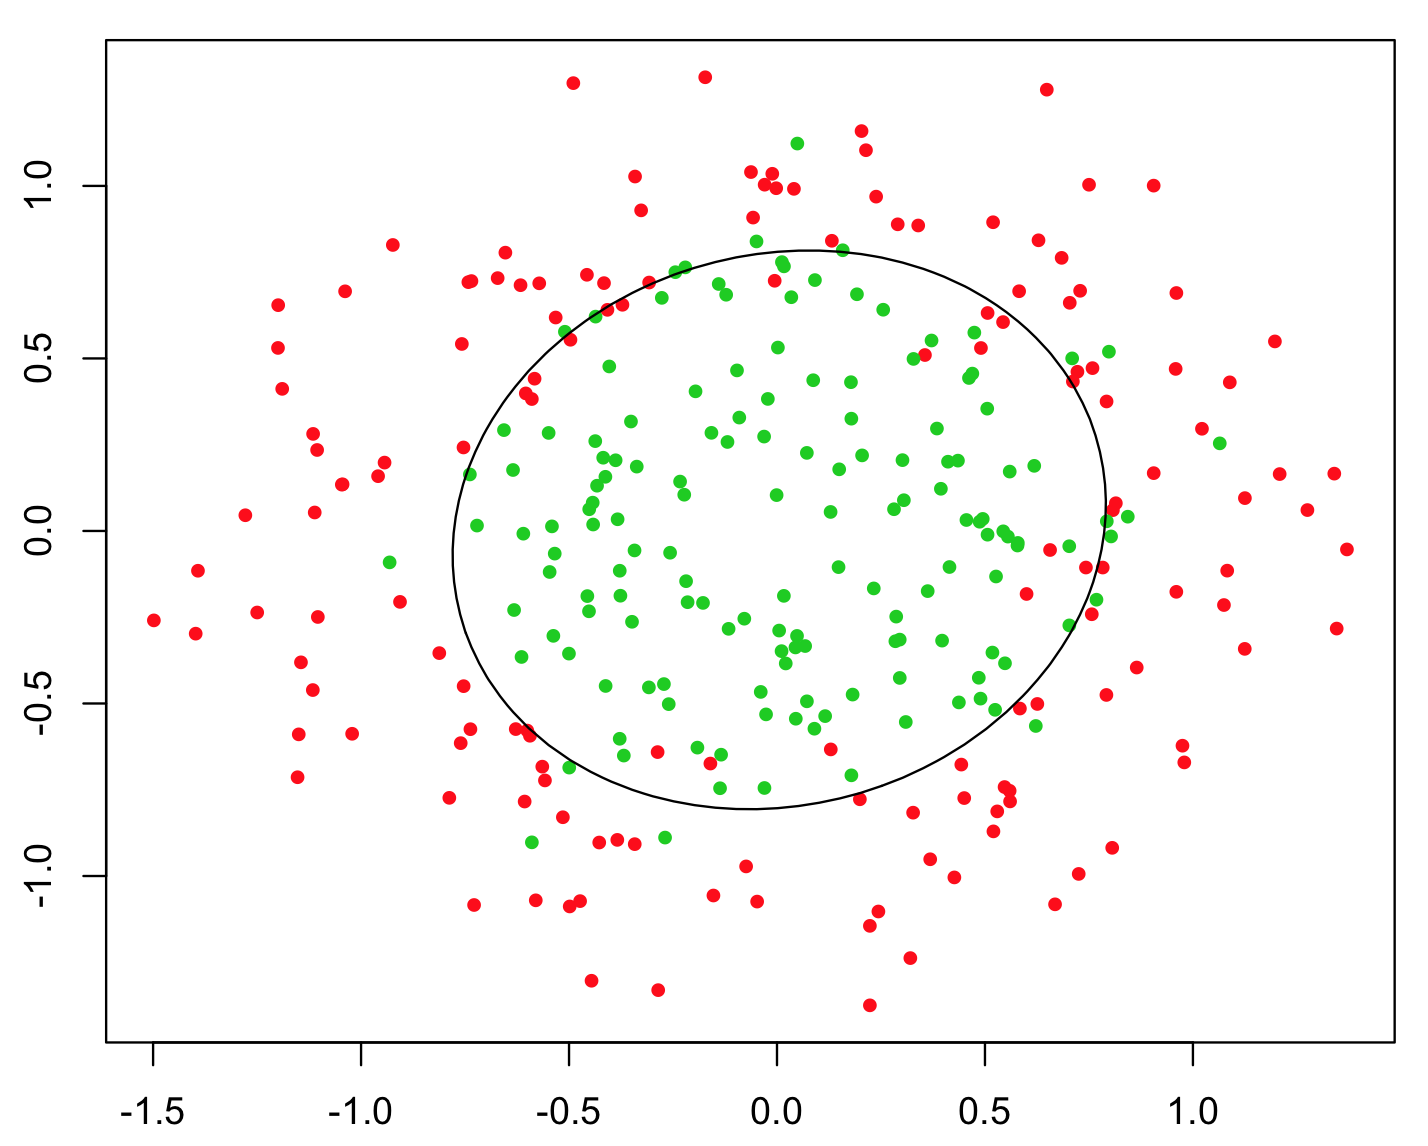
\includegraphics[scale=0.13]{./images/logisticRegression02.png}
                \caption{Example taken from statsblogs.com}
            \end{figure}
        \end{center}
    \end{column}
    \end{columns}
\end{frame}
% -------------------------------------------------------------------------------------------------
\begin{frame}{Linear regression - coding time}
    \begin{itemize}
        \item Let's code logistic regression in \texttt{scikit-learn}
    \end{itemize}
\end{frame}
% -------------------------------------------------------------------------------------------------
%\section{Unsupervised learning}
 %-------------------------------------------------------------------------------------------------
%\section{Reinforcement learning}
% -------------------------------------------------------------------------------------------------
%-----------------------------------------------------------------
\begin{frame}
\Huge{\centerline{Questions?}}
\end{frame}
%-----------------------------------------------------------------
\begin{frame}
\Huge{\centerline{Thank you!}}
\end{frame}
%-----------------------------------------------------------------


\begin{frame}[t, allowframebreaks]
\frametitle{Bibliography}
\bibliographystyle{apalike}
\bibliography{the_bibliography}
\end{frame}

\end{document}
\endinput
%%
%% End of file `example_DarkConsole.tex'.
